%% Standard start of a latex document
\documentclass[letterpaper,10pt]{article}
%% Always use 12pt - it is much easier to read
%% Things written after '%' sign, are ignored by the latex editor - they are how to introduce comments into your .tex source
%% Anything mathematics related should be put in between '$' signs.

%% Set some names and numbers here so we can use them below
\newcommand{\myname}{Group 1} %%%%%%%%%%%%%%% ---------> Change this to your name
% \newcommand{\mynumber}{12345678} %%%%%%%%%%%%%%% ---------> Change this to your student number
% \newcommand{\hw}{1} %%%%%%%%%%%%%%% --------->  set this to the homework number

%%%%%%
%% There is a bit of stuff below which you should not have to change
%%%%%%

%% AMS mathematics packages - they contain many useful fonts and symbols.
\usepackage{amsmath, amsfonts, amssymb}
\usepackage{graphicx}

%% The geometry package changes the margins to use more of the page, I suggest
%% using it because standard latex margins are chosen for articles and letters,
%% not homework.
\usepackage[paper=letterpaper,left=25mm,right=25mm,top=3cm,bottom=25mm]{geometry}
%% For details of how this package work, google the ``latex geometry documentation''.

%%
%% Fancy headers and footers - make the document look nice
\usepackage{fancyhdr} %% for details on how this work, search-engine ``fancyhdr documentation''
\pagestyle{fancy}
%%
%% The header
\lhead{MATH 441} % course name as top-left
\chead{Group Project: Progress Report} % homework number in top-centre
\rhead{ \myname }
%% This is a little more complicated because we have used `` \\ '' to force a line-break between the name and number.
%%
%% The footer
\lfoot{\myname} % name on bottom-left
\cfoot{Page \thepage} % page in middle
%\rfoot{\mynumber} % student number on bottom-right
%%
%% These put horizontal lines between the main text and header and footer.
\renewcommand{\headrulewidth}{0.4pt}
\renewcommand{\footrulewidth}{0.4pt}
%%%


% Some useful macros

\usepackage{amsmath,amssymb,amsthm}
\usepackage{enumerate}

\newcommand{\ZZ}{\mathbb{Z}}
\newcommand{\FF}{\mathbb{F}}
\newcommand{\RR}{\mathbb{R}}
\newcommand{\QQ}{\mathbb{Q}}
\newcommand{\CC}{\mathbb{C}}
\newcommand{\NN}{\mathbb{N}}
\renewcommand\vec{\mathbf}

\newcommand{\st}{\text{ such that } }
\newcommand{\dee}[1]{\mathrm{d}#1}
\newcommand{\diff}[2]{ \frac{\dee{#1}}{\dee{#2}} }
\newcommand{\lt}{<}
\newcommand{\gt}{>}
\newcommand{\set}[1]{\left\{#1 \right\}}


\begin{document}
% Put your answsers as items in this enumerate environment and they will be automatically numbered
\subsection*{FIFA 2026 World Cup Scheduler:} 
For this project, we are looking to tackle the game scheduling problem of the FIFA 2026 world cup. Consider the following pre-emptive schedule from the FIFA website: 
\begin{center}
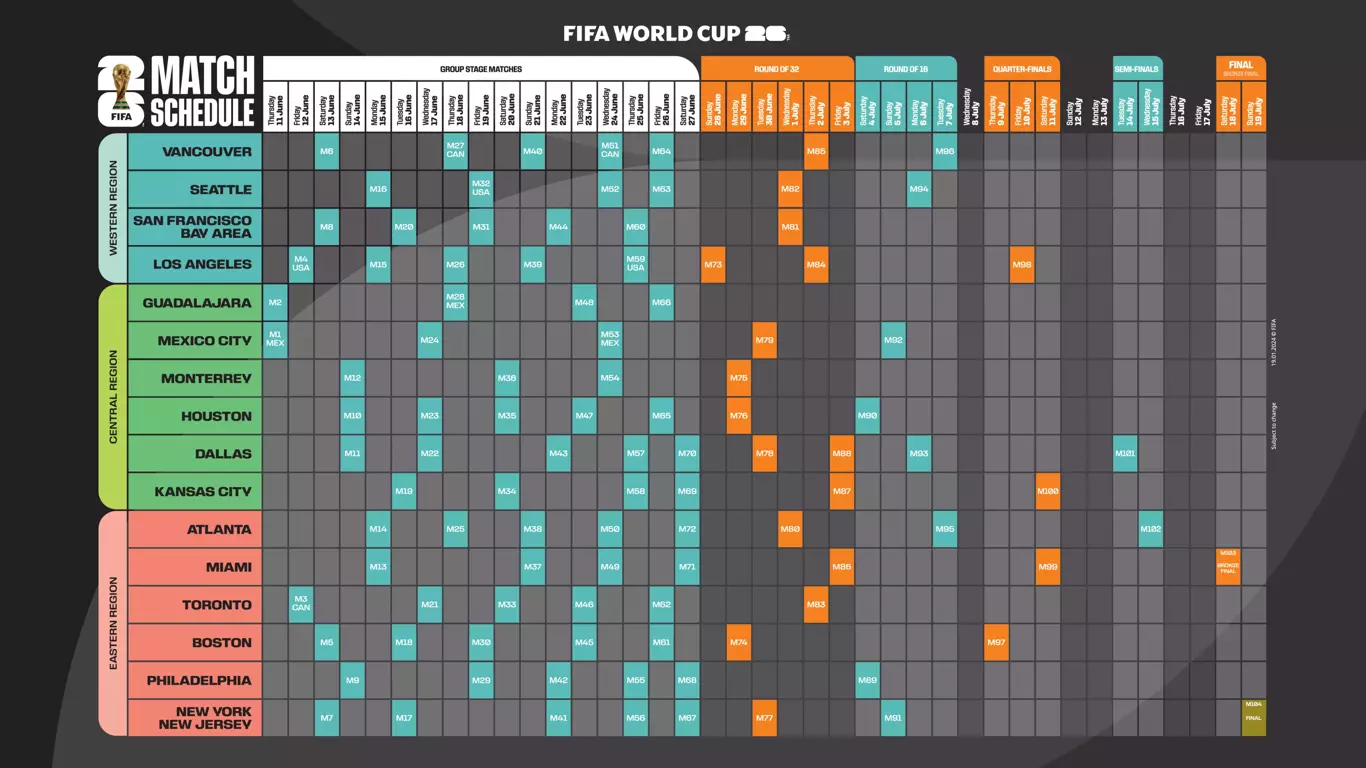
\includegraphics[scale=0.35]{schedule.png}
\end{center}
As can be seen, each game is pre-determined to be played at a certain location within either Canada, the USA, or Mexico. The time and location of the games are locked in, however, the specific teams which will play each game have yet to be scheduled. This is what our project would be looking to determine. Due to the nature of the sport and the popularity of the world cup, it is crucial that the game's schedule is beneficial to both the players, as well as the hosting cities. \\\\
\textbf{Note: }For the purpose of this project, we will only be looking to schedule the group stages. This is because in order to schedule the "round of 32", we must know which teams make it past the group stage. Although it is possible to predict the results of the group stage, that is not within the scope of this project, and is also quite indeterministic. 

\subsubsection*{Constraints:} 
To further specify the problem, we have several constraints that our scheduler must adhere to:
\begin{itemize}
\itemsep0em 
\item 48 unique teams
\item 12 independent groups (4 teams per group)
\item 3 regions (Western has 3 groups, Central has 4 groups, Eastern has 5 groups)
\item 3 Games per team (play all other teams within group once)
\item 3 Days of rest (at least) between games per team
\item Most popular teams play within the bigger stadiums ("most popular" to be defined later on)
\end{itemize}

\newpage
\subsubsection*{Current Approach:} 
The approach we are going to be taking is similar to that of a Sudoku solver. In particular, we will be using techniques from Constraint Satisfaction and Backtracking to recursively check the feasibility of a particular solution, then subsequently "prune out" infeasible solutions from our solution set. Once we have a set of feasible solutions, we can take the "optimal" solution as defined by our objective function. For example, we can model our set of feasible solutions as a depth-first search tree:
\begin{center}
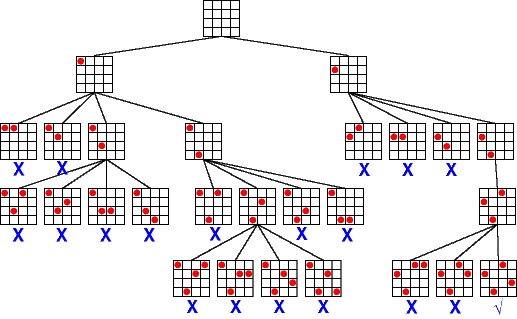
\includegraphics[scale=0.8]{backtrack.png}
\end{center}
We can assume that the root is the initial state of the schedule (empty). At each layer, we add a pair of two teams to any particular match time slot, and check if that pairing is considered feasible by our constraints. If it is, then we can recursively add a second pair of teams to a new match slot and again check if it is feasible. If it is not feasible, then we can "prune" out that branch such that no further recursions are made with those two teams within that initial slot. This way, we are only left with branches that are considered feasible, and subsequently leaf nodes which contain feasible solutions. Once we have a set of all feasible solutions, we can maximize our objective function over all solutions such that we keep the solution which produces the highest revenue/popularity for FIFA (function will be defined in the next section). \\
\\
Our data structure will be similar to the above diagram, where each node of the tree will be an $nd$-array containing the current feasible schedule, and each branch below will be a progression of that schedule. To begin, the root node will have many possible children (since the first match can likely be almost all pairings), however as the tree progresses, the nodes will get pruned out.\\
\\
This approach is essentially a glorified brute-force search, however, due to the small input space combined with the tight constraints for the teams, we believe a brute force approach won't be much of a computational burden.

\newpage
\subsubsection*{Technical Specifics:} 
Let's define the following variables: 
\begin{itemize}
\item $d_i$ corresponds to day $i$ of the group stages. Thus, $d_i \in \{d_0, ..., d_D \}$ where we have $D$ days total.
\item $s_j$ corresponds to stadium $j$ within the regions. Thus, $s_j \in \{s_0, ..., s_S \}$ where we have $S$ stadiums total.
\item $t_k$ is a unique team. Thus, $t_k \in \{t_0, ..., t_T \}$ where we have $T$ teams total.
\item $g_m$ is a unique group containing $t_{4m}, t_{4m+1}, t_{4m+2}, t_{4m+3}$ where $m \in \{0, ..., \frac{T}{4} \}$.
\item $m_n$ is a unique team matching where $m_n \in \{ m_0, ..., m_M\}$ where we have $M$ unique match-ups total.
\item $m(t_k, t_l)$ is a mapping function that maps pairs of teams to matches. If a match exists, return $m_n$, else, return $0$. Conversely, we can map $t(m_n)$ that returns the teams $t_k, t_l$ corresponding to the certain match.
\item $X(d_i, s_j, t_k, t_l) \in \{0,1\}$ where $1$ if team $t_k$ plays team $t_l$ on day $d_i$ at stadium $s_j$, else $0$.

\end{itemize}
~\\
Additionally, we can define the given constraints in terms of the above variables:
\begin{itemize}
\item Restrict schedule to only valid official game days:
\begin{align*}
\text{for all $i,j,k,l$}; \quad X(d_i, s_j, t_k, t_l) = 0 \quad \text{if not aligned with official FIFA schedule}
\end{align*}
\item Each team plays once per day:
\begin{align*}
\text{for all $d,t$}; \quad \sum_{j = 0}^S \sum_{l = 0}^T X(d, s_j, t_k, t) &= 1 \\
\text{for all $d,t$}; \quad \sum_{j = 0}^S \sum_{k = 0}^T X(d, s_j, t, t_l) &= 1
\end{align*}
\item $1$ match per day day, per stadium:
\begin{align*}
\text{for all $d,s$}; \quad \sum_{k = 0}^T \sum_{l = 0}^T X(d, s, t_k, t_l) = 1
\end{align*}
\item $3$ days of rest at least per team in between games:
\begin{align*}
&\text{if} \quad X(d_i, s_j, t_k, t_l) = 1, \quad \text{then} \\
&\qquad \text{for all $s$} \\
&\qquad \qquad \left[ X(d_{i + 1}, s, t', t) + X(d_{i + 2}, s, t', t) + X(d_{i + 3}, s, t', t)\right] = 0 \quad \text{for all $t$ and} \quad t' \not\in \{t_k, t_l \} \\
&\qquad \qquad \left[ X(d_{i + 1}, s, t, t') + X(d_{i + 2}, s, t, t') + X(d_{i + 3}, s, t, t')\right] = 0 \quad \text{for all $t$ and} \quad t' \not\in \{t_k, t_l \}-
\end{align*}
\item Each team can only play another team within it's group (and not itself):
\begin{align*}
\text{if} \quad X(d_i, s, t_k, t_l) = 1, \quad \text{then}, \quad t_k, t_l \in g_m \quad \text{and} \quad t_k \neq t_l
\end{align*}
\end{itemize}
Once we have the variables and constraints, we can define the objective function as 
\begin{align*}
\text{maximize} \quad \sum_{l = 0}^T \sum_{k = 0}^T \sum_{j = 0}^S \sum_{i = 0}^D X(d_i, s_j, t_k, t_l) \cdot r(d_i, s_j, t_k, t_l)
\end{align*}
where $r(d_i, s_j, t_k)$ is a revenue function which returns the estimated revenue generated by team $t_k$ playing at stadium $s_j$ on day $d_i$. We will determine $r$ through external data such as international popularity rankings of specific teams, stadium capacity numbers, and nationality bias. 
\end{document}
